\chapter{Implementation}
This chapter discusses the implementation details of the proposed mobile application. First, the \gls{har} stages will be discussed. That includes the data gathering from the projects' participants as well as data prepossessing and training a classifier. Next, the specifics of the mobile application itself will be discussed such as database and overall system design implementation.

\section{The mobile application}
       
    \subsection{MVP and Dependency Injection}
    As discussed before, the implementation of the mobile application is following the \gls{mvp} software pattern, which allows for the clear separation of code concepts (see section \ref{section:architectural-design}). To better satisfy the requirements discussed in section \ref{section:system-quality-attributes}, \gls{mvp} is combined with a Dependency Injection (DI) principle. What \gls{di} do is shifting the responsibility of one class to create its dependencies to another class. For example, class Car requires class Engine as a parameter. Instead of creating a new instance of class Engine when class Car is created it is simply provided as a constructor parameter in class Car's constructor (see listing \ref{di-car-example}).
    
    Dagger\footnote{\url{https://github.com/google/dagger}} is a framework that utilises the \gls{di} principle in the form of \textit{Component} and \textit{Module} classes. A module creates the necessary dependencies (e.g. object of class B) whereas the Component class determines where those dependencies will be "injected" (e.g. satisfy dependence's in class A). A concrete example of \gls{di} can be seen in Listing \ref{di-example}. In this example, the \textbf{LoginFragment} (e.g. the login screen) requires an object of type \textit{\textbf{"ILoginPresenter"}} to function. The method \textit{\textbf{"satisfyDependencies()"}} provides the dependencies to the class (e.g. externally). All of the dependencies of the Login screen are provided from a Dagger module named \textit{\textbf{"AuthModule"}} which is responsible for providing and creating the concrete implementation of the above interface (e.g. ILoginPresenter). The full code of \textit{\textbf{"AuthModule"}} as well as \textit{\textbf{"AuthComponent"}} can be seen in Appendix \ref{chapter:dagger-component-module}.   
    
    
\begin{lstlisting}[caption= DI example, label=di-car-example,frame=tlrbr,basicstyle=\small,captionpos=b]
    class Car{
        Engine engine;
            Car(Engine engine){
                this.engine = engine;
            }
       }
    }
\end{lstlisting}
        
    Combining the \gls{mvp} design pattern with dependency injection framework such as Dagger brings a lot of advantages for the software product. Firstly, the software becomes more loosely coupled as the \gls{mvp} enforces the use of interfaces and Dagger is responsible for injecting the concrete implementation of those interfaces where required. Secondly, it allows for logically structuring the codebase. For example, a common approach when using both \gls{mvp} and Dagger is to create a directory for each one of the mobile screens (see figure \ref{fig:app-directory-structure}) containing the necessary \gls{mvp} classes such as \textit{\textbf{Presenter}} and \textit{\textbf{Model}} and the as well as Dagger's \textit{\textbf{Module}} and \textit{\textbf{Component}} to handle the \gls{di} process.
    
    \begin{wrapfigure}{RI}{0.3\textwidth}
        \begin{center}
            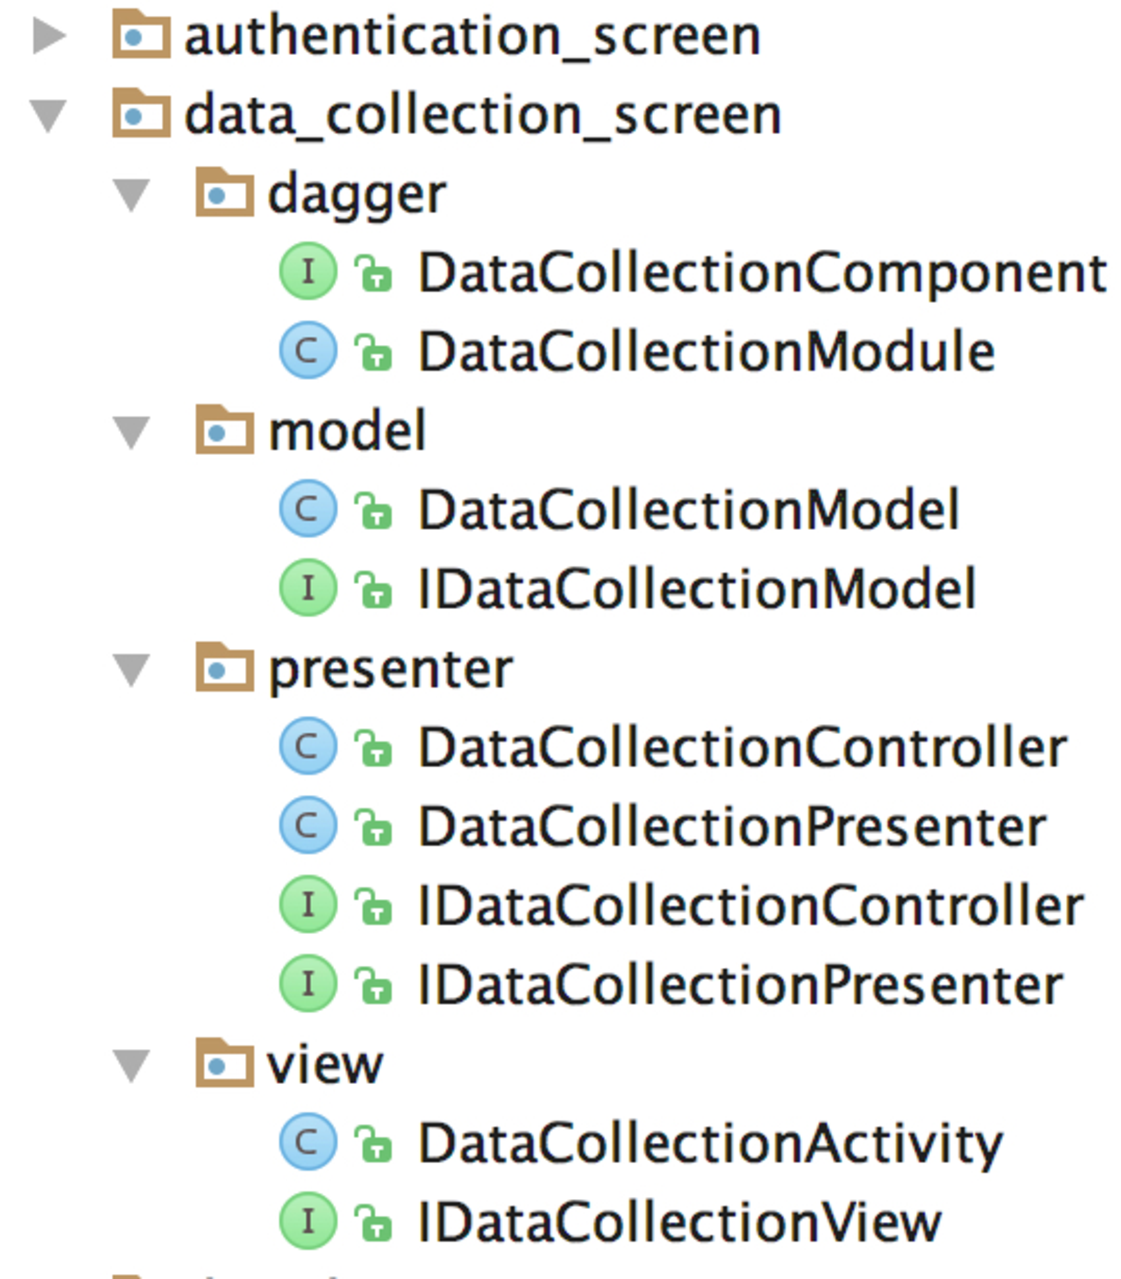
\includegraphics[width=0.3\textwidth]{app-directory-structure}
        \end{center}
    \caption{Data collection screen directory structure}
    \label{fig:app-directory-structure}
    \end{wrapfigure}
   
    
    \subsection{Realm Database}
    
    \subsection{Data collection service}
    
    \subsection{Active Minutes service}
    


\section{Human Activity Recognition}
In order for the system to take actions such as notifying the user for a prolonged periods of inactivity or sending a notification when a \gls{pa} goal is achieved, the application needs to recognise human activities (i.e. walking and running). Implementation of the \gls{har} system will be discussed bellow.

    \subsection{Data Collection}
    One of the key stages in the development process of a typical supervised (online) \gls{har} system is the data collection stage. A labelled dataset is needed in order to train a model (or also called classifier). The produced model can classify an "unseen" (or unlabeled) data to a specific activity (i.e. walking or being static).
    
    \subsubsection*{Setting and project participants}
    The data needed to train the model in this work was collected from 3 fellow students in a controlled environment. Each one of the project participants was equipped with a device running partially implemented \textit{"Active Minutes"} application (e.g. only the \textit{"Data Collection screen"} see \ref{fig:data-collection-screen-design}). Before performing the data collection process, the participants had to, first, select the activity they will perform from a list of activities and then press the Start button on the application's UI in order to start the data collection process. The location of the device during the recording was chosen to be the front pants pocket. This location has been found to be the optimal position for \gls{har} (see \ref{section:non-commercial-har-systems}). All of the participants recorded 3 minutes of each one of the following activities: \textit{walking}, \textit{running}, \textit{cycling} and \textit{static}. To avoid any unwanted information during the recording stage, the first and the last 7 seconds of each activity was removed since it contained noise information such as the linear acceleration taking place when the device was put in and pulled out of participants pockets. That was pragmatically done and no direct human intervention was needed to further filter the data.
    
    \subsubsection*{Recorded data and type of device used}
    When all of the required data was collected, it was converted into a WEKA ARFF file format by pressing the "EXPORT" button on the Data Collection screen. The ARFF file was stored on the device's external memory (e.g. SD card). A sample of the produced ARFF file can be seen in Listing \ref{weka-arff-code}. A dataset containing ~720 labelled data points (or a total of ~36 minutes of data) was produced as a result of the data collection process. 
    
   
    
\begin{lstlisting}[caption=WEKA ARFF file extract,
label=weka-arff-code,captionpos=b, frame=single,basicstyle=\small,float,floatplacement=H,breaklines=true]
@relation HAR
    
@attribute accX__fft1 numeric
@attribute accX__fft2 numeric
@attribute accX__fft3 numeric
@attribute accX__fft4 numeric
@attribute accX__fft5 numeric
@attribute accY__fft1 numeric
@attribute accY__fft2 numeric
@attribute accY__fft3 numeric
@attribute accY__fft4 numeric
@attribute accY__fft5 numeric
@attribute accZ__fft1 numeric
@attribute accZ__fft2 numeric
@attribute accZ__fft3 numeric
@attribute accZ__fft4 numeric
@attribute accZ__fft5 numeric
@attribute accM__fft1 numeric
@attribute accM__fft2 numeric
@attribute accM__fft3 numeric
@attribute accM__fft4 numeric
@attribute accM__fft5 numeric
@attribute class {walking,running,static,cycling}
    
@data
9,-76,-834,25,22,4,-1,-401,-190,-3,3,5,-213,-94,-45,2,-50,-49,-15,18,walking
-0,-184,140,4,-34,-2,13,45,63,-8,0,51,-68,-30,-72,1,-52,15,-51,63,walking
-1,-13,-30,3,2,3,-18,-2,3,-21,-1,2,-4,-9,-1,-2,33,3,16,20,walking
0,-16,-17,-22,6,-3,-6,-8,-16,-3,-15,-2,12,-5,9,8,8,37,38,-18,walking
-6,-22,14,-54,1,14,8,27,9,60,-22,-31,-11,-11,4,-7,1,0,-3,-39,running
-3,-11,-35,-3,-53,-13,-45,23,-57,17,-2,52,13,58,15,22,48,-36,25,-50,running
3,7,-11,27,-41,-19,-31,-53,-107,10,0,-42,22,-42,3,20,34,-26,76,-104,running
-3,37,34,9,58,0,30,97,-74,83,4,-13,-39,40,26,-4,15,-10,27,-26,cycling
-1,-91,-131,-121,-58,-4,6,-66,22,70,3,-30,-76,-63,-30,-1,-39,-10,-39,-76,cycling
1,-54,-41,-180,114,-3,4,-21,78,-188,3,8,-56,-19,70,0,-38,22,-83,103,cycling
0.3,0,-1,1,-1.4,0,1,-1,0,0,0,-1,0,0,0,0,0,0,0,0,static
0,-6,48,-8,0,0,-6,-21,2,5,0,-1,42,-6,0,0,0,-1.5,0,-1.6,static
-0.3,8,-4,3,-4,0.1,6,-4,2,-3,0,2,-2,2,-1,0,0.2,1,-0.4,0.2,static
\end{lstlisting}
    
    The device used to collect the data was \textit{OnePlus One} equipped with low-power high performance 3-axes accelerometer \footnote{\url{http://www.st.com/en/mems-and-sensors/lis3dh.html}}. As for the sampling frequency (SF) of the sensor, the Android Operating system provides a total of four different sampling frequencies for reading the accelerometer sensor, namely \textit{NORMAL: 5 Hz}, \textit{UI: 16 Hz}, \textit{GAME: 50 Hz}, and \textit{FASTEST}. The latter has been chosen for the SF of the built-in accelerometer as it has produced good results in \citet[3-5]{lee2016}. According to the Google's documentation \textit{FASTEST} SF depends on the hardware of the device \citep{googlesensormanager2017}. In this case, the SF was \textbf{115} Hz. 
    
    \subsection{Training the classifier}
    THE APPLICATION CREATES THE CLASSIFIER UPON THE FIRST LAUNCH
    
    
    